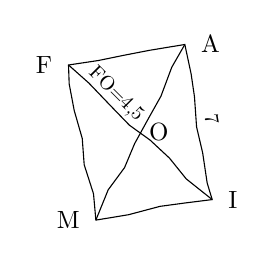
\begin{tikzpicture}[rotate=10,every node/.style={scale=0.9},scale=1]

\coordinate (F) at (0,0);
\coordinate (A) at (1.5,0);
\coordinate (I) at (1.5,-2);
\coordinate (M) at (0,-2);
\coordinate (O) at (0.75,-1); %le centre du rectangle

\draw[decorate,decoration={random steps,amplitude=1pt,segment length=10pt}] (F) node [left=3pt]{F}--(A) node [right=3pt]{A} --(I) node [right=3pt] {I}--(M) node [left=3pt] {M}--cycle;
\draw [decorate,decoration={random steps,amplitude=1pt,segment length=10pt}] (F)--(I) (A)--(M);
\node at (O)[right]{O}; 
\node at (.53,-.47)[rotate=-45,scale=0.8]{FO=4,5};
\path (A)--(I) node[midway,above,rotate=-80,scale=0.8]{7};
%\path (T)--(O) node[midway,above,rotate=-5]{OT=2};

\end{tikzpicture}
